\chapter{Introduction to Photonics}
\minitoc
\pagebreak
\section{Measurement of light's power}
There are two main ways of quantifying an electromagnetic waves power: radiometric and photometric.
Photometric is how much power will be seen by the human eye, while radiometric is a direct measurement of the waves power.
In these cases, light is defined as being in the visible spectrum although radiometry covers ultraviolet and infrared radiation.
The photometric measurement uses a standard responsivity of the human eye which is defined by the $V(\lambda)$ curve  shown in figure \ref{fig:eye}.
\begin{figure}[H]
	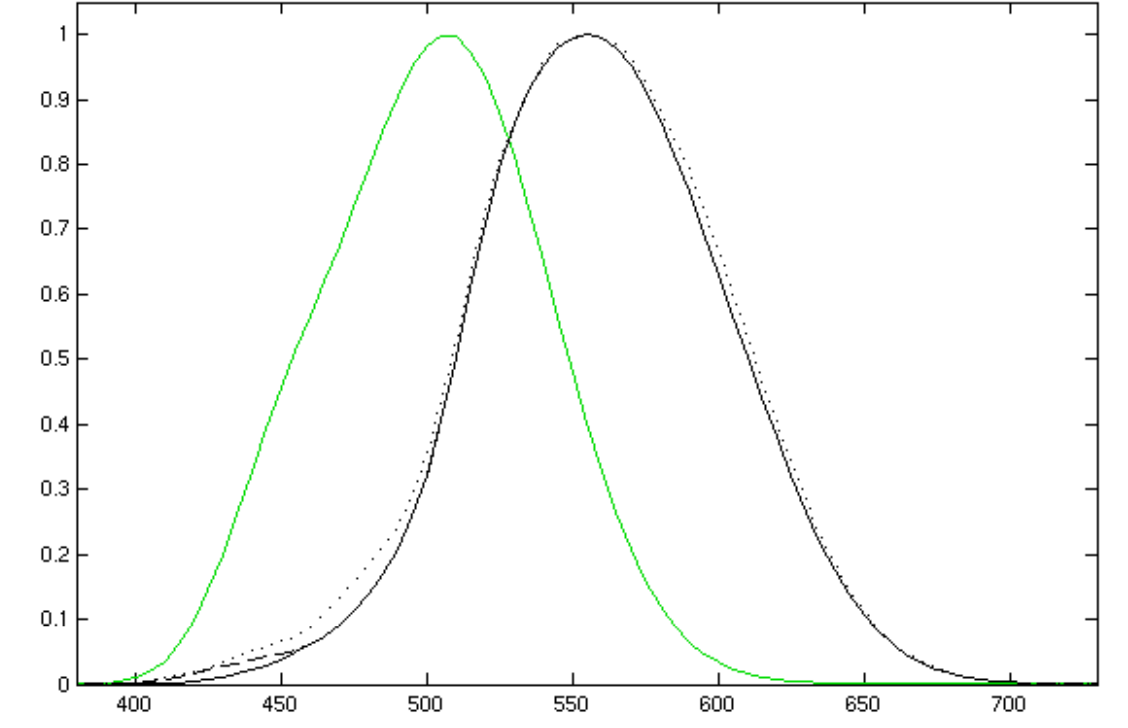
\includegraphics[width=\linewidth]{eye}
	\caption{The graph shows the curve for the photopic response, the black line, and the scotopic response, the green line, of a standard human eye}
	\label{fig:eye}
\end{figure}
There are two main types of responses: the scotopic, the green line, and this is for an eye adapted to the dark, and the photopic, the black line, for an eye adapted to bright light.
The radiant flux spectral distribution, $\phi_e(\lambda)$, can be used to calculate the luminious flux (the photometric version), $\phi_v$ using 
\begin{equation}
\phi_v = K\int{V(\lambda)\phi_e(\lambda)d\lambda}.
\label{eq:luminous}
\end{equation}
$K$ is the spectral luminous efficiency defined as 683 lmW$^{-1}$.
\section{Polarisation}
For the most part the basics of polarisation are the same as in \textit{Wave Optics} although the definition of circularly polarised light may be different.
 For example, right hand circularly polarised light is defined as when you look towards the source with light coming towards you, you can curl your right hand in the direction of the rotation with the thumb pointing towards you. %This is terrible, I'm sorry
 The same applies for left hand circularly polarised light, although with the left hand.
 \\
 The intensity reflection coefficient, $R$, for incident light, $\theta_i$ = 0, is
 \begin{equation}
 R = \left(\frac{n_1-n_2}{n_1+n_2}\right)^2
 \end{equation}
 


